% !TeX document-id = {5530719d-34df-4dd8-b4b5-e6ed092c2b36}
% !TeX program = pdflatex
% !BIB program = biber
\documentclass[sigconf,natbib=false]{acmart}

% Imports Ahoy

%\usepackage[dvipsnames]{xcolor}
%\usepackage{graphicx}
\usepackage{tikz}
\usepackage{varwidth}
\usetikzlibrary{arrows.meta, calc, fit, positioning}

\usepackage[title]{appendix}

\usepackage{etoolbox}
\usepackage[binary-units, per-mode=symbol]{siunitx}
\robustify\bfseries
\robustify\emph
%\robustify\uline
\sisetup{detect-all, range-phrase=--, range-units=single, detect-weight=true,detect-inline-weight=math, table-format=1.3}

\makeatletter
\let\MYcaption\@makecaption
\makeatother

\usepackage[font=footnotesize]{subcaption}
\usepackage{awesomebox}

\makeatletter
\let\@makecaption\MYcaption
\makeatother

%\usepackage[basic]{complexity}
\usepackage[super,negative]{nth}

\usepackage[british]{babel}
\usepackage{csquotes}
\usepackage{pifont}

\usepackage{booktabs}
%\usepackage[
%activate={true,nocompatibility},
%final,
%tracking=true,
%kerning=true,spacing=true
%]{microtype}
%\microtypecontext{spacing=nonfrench}

\usepackage[maxnames=2,maxbibnames=99,mincrossrefs=99,sortcites,style=numeric-comp
%,backend=biber
]{biblatex}
\addbibresource{papers-off.bib}
\addbibresource{confs-off.bib}
\addbibresource{books-off.bib}
\addbibresource{rfc.bib}
\addbibresource{misc.bib}

%\DeclareFieldFormat[inproceedings]{doi}{}
%\DeclareFieldFormat[article]{doi}{}
%\DeclareFieldFormat*{url}{}
%\DeclareFieldFormat[online]{url}{\mkbibacro{URL}\addcolon\space\url{#1}}
%\DeclareFieldFormat[report]{url}{\mkbibacro{URL}\addcolon\space\url{#1}}

%picky abt et al.
\usepackage{xpatch}

\usepackage{url}
\usepackage{hyperref}
\usepackage[nameinlink]{cleveref}
\newcommand{\crefrangeconjunction}{--}
\crefname{table}{table}{tables}

\DefineBibliographyStrings{english}{%
	andothers = {\emph{et al}\adddot}
}
\DeclareFieldFormat[inproceedings]{url}{}
\DeclareFieldFormat[article]{url}{}
%\DeclareFieldFormat[inproceedings]{doi}{}
%\DeclareFieldFormat[article]{doi}{}
%\DeclareFieldFormat[inproceedings]{editor}{}
%\DeclareFieldFormat[proceedings]{editor}{}
%\DeclareFieldFormat[article]{editor}{}

\newcommand{\fakepara}[1]{\noindent\textbf{#1:}}

% Official colours!

\definecolor{uofguniversityblue}{rgb}{0, 0.219608, 0.396078}

\definecolor{uofgheather}{rgb}{0.356863, 0.32549, 0.490196}
\definecolor{uofgaquamarine}{rgb}{0.603922, 0.72549, 0.678431}
\definecolor{uofgslate}{rgb}{0.309804, 0.34902, 0.380392}
\definecolor{uofgrose}{rgb}{0.823529, 0.470588, 0.709804}
\definecolor{uofgmocha}{rgb}{0.709804, 0.564706, 0.47451}

\definecolor{uofglawn}{rgb}{0.517647, 0.741176, 0}
\definecolor{uofgcobalt}{rgb}{0, 0.615686, 0.92549}
\definecolor{uofgturquoise}{rgb}{0, 0.709804, 0.819608}
\definecolor{uofgsunshine}{rgb}{1.0, 0.862745, 0.211765}
\definecolor{uofgpumpkin}{rgb}{1.0, 0.72549, 0.282353}
\definecolor{uofgthistle}{rgb}{0.584314, 0.070588, 0.447059}
\definecolor{uofgpillarbox}{rgb}{0.701961, 0.047059, 0}
\definecolor{uofglavendar}{rgb}{0.356863, 0.301961, 0.580392}

\definecolor{uofgsandstone}{rgb}{0.321569, 0.278431, 0.231373}
\definecolor{uofgforest}{rgb}{0, 0.317647, 0.2}
\definecolor{uofgburgundy}{rgb}{0.490196, 0.133333, 0.223529}
\definecolor{uofgrust}{rgb}{0.603922, 0.227451, 0.023529}

% End Imports

%\usepackage[english]{babel}
\usepackage{blindtext}

% Copyright
%\renewcommand\footnotetextcopyrightpermission[1]{} % removes footnote with conference info
%\setcopyright{none}
\setcopyright{acmcopyright}
%\setcopyright{acmlicensed}
%\setcopyright{rightsretained}
%\setcopyright{usgov}
%\setcopyright{usgovmixed}
%\setcopyright{cagov}
%\setcopyright{cagovmixed}

%\settopmatter{printacmref=false, printccs=false, printfolios=true}
\settopmatter{printfolios=true}

% DOI
\acmDOI{12345}

% ISBN
\acmISBN{67890}

%Conference
\acmConference[SOSR '21]{Symposium of SDx Research 2021}{September \numrange{13}{14}, 2021}{Online}
\acmYear{2021}
%\copyrightyear{}

%% {} with no args suppresses printing of the price
\acmPrice{15.00}

\newcommand{\approach}{On Path Learning}
\newcommand{\approachshort}{OPaL}

\makeatletter\let\expandableinput\@@input\makeatother
\newcommand{\cmark}{\ding{51}}%
\newcommand{\xmark}{\ding{55}}%

\newcounter{insightc}
\newenvironment{insight}
	{
		\begin{tipblock}\refstepcounter{insightc}\textbf{Insight \theinsightc:}\em
	}
	{
		\end{tipblock}
	}

\begin{document}
	\title{Revisiting~the~Classics: Online~RL~in~the~Programmable~Dataplane}
	
%	\titlenote{Produces the permission block, and copyright information}
	%\subtitle{Extended Abstract}
	
%	\author{Paper \# XXX, XXX pages}
	 \author{Kyle A. Simpson}
	 \orcid{0000-0001-8068-9909}
	 \affiliation{%
	   \institution{University of Glasgow}
	   \city{Glasgow} 
	   \country{Scotland}
	 }
	 \email{k.simpson.1@research.gla.ac.uk}
	 \author{Dimitrios P. Pezaros}
\orcid{0000-0003-0939-378X}
	 \affiliation{%
	\institution{University of Glasgow}
	\city{Glasgow} 
	\country{Scotland}
}
\email{Dimitrios.Pezaros@gla.ac.uk}
	
% The default list of authors is too long for headers}
\renewcommand{\shortauthors}{Simpson \emph{et al}.}
	
\begin{abstract}
?? In-NIC execution allows clever use of resources to bring action compute latency  from \SI{1}{\milli\second} to \SI{50}{\micro\second} (2 orders of magnitude!) in real-world policies for DDoS detection/prevention control.
\end{abstract}

\begin{CCSXML}
	<ccs2012>
	<concept>
	<concept_id>10003033.10003068.10003069</concept_id>
	<concept_desc>Networks~Data path algorithms</concept_desc>
	<concept_significance>500</concept_significance>
	</concept>
	<concept>
	<concept_id>10003033.10003099.10003102</concept_id>
	<concept_desc>Networks~Programmable networks</concept_desc>
	<concept_significance>500</concept_significance>
	</concept>
	<concept>
	<concept_id>10003752.10010070.10010071.10010261</concept_id>
	<concept_desc>Theory of computation~Reinforcement learning</concept_desc>
	<concept_significance>300</concept_significance>
	</concept>
	<concept>
	<concept_id>10010147.10010257.10010258.10010261</concept_id>
	<concept_desc>Computing methodologies~Reinforcement learning</concept_desc>
	<concept_significance>500</concept_significance>
	</concept>
	</ccs2012>
\end{CCSXML}

\ccsdesc[500]{Networks~Data path algorithms}
\ccsdesc[500]{Networks~Programmable networks}
\ccsdesc[500]{Computing methodologies~Reinforcement learning}

%\keywords{ACM proceedings, \LaTeX, text tagging}
	
\maketitle

\setlength{\aweboxleftmargin}{0.12\linewidth}
\setlength{\aweboxcontentwidth}{1.97\linewidth}
	
\section{Introduction}
?? REDO ME

Automatic optimisation, control, and defence of networks are at last becoming commonplace. Data-driven networking has led the charge in traffic optimisation, congestion control and packet classification via adaptive techniques such as Reinforcement Learning (RL), where every change and its measured effects further improve future decisions. Considering that the network evolves in its use and deployed protocols, this flexibility is essential. Yet data-driven methods suffer from a key weakness: they are dependent on both the recency and accuracy of input state. An out-of-date view of the world will lead to suboptimal choices, as will long processing times. These can result in worse performance and slower adaptation to the evolving network.

Programmable data-planes and in-switch compute, then, hold promise for integrating these new techniques in a feasible and efficient manner (beyond dedicated servers or virtualised network functions). For RL, key tasks include policy evaluation, online training, state collection, and action execution -- each of these introduces some degree of sensitivity to state accuracy. Ideally then, all logic would run on these programmable devices. Yet, there is often a finite budget in microcode/FPGA space, per-packet processing times, and available cores for execution. Moreover, necessary hardware, such as floating-point units, is unavailable in almost all cases.

The precise costs and trade-offs which operators and designers must make have yet to be identified. This follows from a design space explosion induced by many necessary workarounds. For instance, quantisation or fixed-point arithmetic will allow training and control on all devices, but introduces further questions: what degree of quantisation is most appropriate? What effect would this have on training accuracy, communications cost, or storage requirements? More concerns arise when we consider core allocation, local vs. distributed training, and reliable lightweight communication in multi-agent scenarios. In all cases, network operators will not consider tools which affect underlying traffic.

I aim to examine the effects of these choices on an existing RL-based DDoS attack mitigation system. To protect legitimate traffic, this controls packet drop and filtering for each flow using individual metrics observed by RL agents at ingress routers, and load measurements from several points along the path taken by the flow in question. The examined metrics include the throughput and latency of its individual components alongside system metrics: flow arrival-to-judgement time, and knowledge propagation time. Beyond this, it's crucial to identify what we can implement on pure P4-capable hardware. While extensions to P4 are fairly common in commodity hardware, the need for full design access (as in NetFPGA) or Micro-C (as in Netronome SmartNICs) represent a break from the clean, loop-free semantics of P4. As the market matures, these may represent different feature classes and price points.

I will discuss early development efforts (including challenges and results) on the Netronome Agilio SmartNIC, which supports the P4 language as well as some degree of arbitrary microcode. I intend to present how reinforcement learning execution and network telemetry will differ in the above metrics when compared to a vNF-based deployment (i.e., software on external commodity servers).

This paper contributes:
\begin{itemize}
	\item An analysis of why in-NIC RL is best-placed to interact with the network, and how classical RL methods and quantisation ensure computational feasibility (\cref{sec:motivation}),
	\item \emph{\approachshort{}}: a general-purpose in-NIC RL agent which scales with allocated device resources to meet latency or throughput demands (\cref{sec:design}),
	\item Potential integrations of \approachshort{} with state-of-the-art PDP applications to perform fully in-NIC, automated DDoS mitigation and ?? OTHER THING (\cref{sec:potential-integrations}),
	\item In-depth evaluation of how our approach affects carried dataplane traffic, performs under different policy sizes, and improves upon explicit offloading to produce a \SI{0}{$\times$} latency reduction (\crefrange{sec:evaluation}{sec:results}). ??actual val
\end{itemize}

\section{Background and Motivation}\label{sec:motivation}
?? RL~\parencite{RL2E}

?? Use this to explain differences between the modern state of the art and older works.

?? Probably give a rough introduction to the algorithm, show what arithmetic operations are needed---particularly when using Qm.n fixed point.

?? Tile coding requires div, though can be simplified using binary tile widths (relates down to bitshifts). What other ops?

?? Explain how it is an embarrassingly parallel problem? Or at least very amenable to partition-aggregate.

?? Critical section around shared writeback loc, but individual work items are disjoint in their input data (particularly useful for updates).

\begin{insight}
	Classical RL methods are computationally simple to update online, and inference and learning are embarrassingly parallel.
\end{insight}

\fakepara{Reinforcement learning in asynchronous environments}
RL techniques allow an \emph{agent} to learn how to iteratively interact with a system in an optimal fashion.
However, there is some degree of divergence between their theory and implementation.
Consider \cref{fig:state-slip}: the traditional formulation of a Markov decision process assumes that an agent receives a new view of the world's state at fixed time intervals, and then decides upon and executes an action instantly.
The reality is that state information takes time to traverse the network, service times are offset by how quickly hosts respond to interrupts and deserialise requests, and action preference lists are often computed via expensive policy approximations.
Action installation also incurs costs in fields such as network administration, initially to contact the controller and then for those actions to be installed via the control plane.

These delays (and variance thereof) add noise to the state-action mapping being learned, which has a potent reduction to learning rate and final accuracy, even for simple grid world tasks according to \textcite{DBLP:journals/firai/TravnikMSP18}.
They in turn show that reordering algorithmic steps can reduce these costs for online 1-step algorithms, but that reducing this further requires detailed agent-environment co-design.
This principle has influenced the design of real network use cases, such RL-based congestion-control algorithms~\parencite{DBLP:journals/corr/abs-1910-04054}, showing that asynchrony is necessary for high-speed applications.
Achieving this often requires that state measurements are combined or coalesced~\parencite{DBLP:journals/corr/abs-1910-04054,DBLP:journals/tnsm/SimpsonRP20} while expensive computations are ongoing.
`Stopping the world' in the algorithmic sense causes significant performance degradation, as inference takes up to \SI{30}{\milli\second} in the above work on congestion control, or any time-sensitive control problems.

\begin{figure}
	\begin{subfigure}{0.45\linewidth}
		\resizebox{\linewidth}{!}{
			\centering
			\begin{tikzpicture}
				\node[circle, draw] (state) {$S$};
				\node[circle, draw] (state') at ($(state) + (0, -2)$) {$S'$};
				
				\node (agent) at ($(2, 0) + (state)$) {Agent};
				\node[below of=agent] (action) {Action $A$};
				
				\node[right of=state'] {$+ R$};
				
				\draw[->] (state) -- (state') node[midway, right] {$A$};
				
				\draw[dotted, ->, bend left = 30] (state) -- (agent);
				\draw[->] (agent) -- (action);
				\draw[dotted, ->] (action) -- (state);
		\end{tikzpicture}}
		\caption{Theory: state measurement, action computation, and learning are zero-cost.}
	\end{subfigure}
	\begin{subfigure}{0.45\linewidth}
		\resizebox{0.75\linewidth}{!}{
			\centering
			\begin{tikzpicture}
				\node[circle, draw] (state) {$S$};
				\node[circle, draw] (state') at ($(state) + (0, -1.5)$) {$S'$};
				\node[circle, draw] (state'') at ($(state') + (0, -1.5)$) {$S''$};
				
				\node (agent) at ($(2, 0) + (state)$) {Agent};
				\node[below of=agent] (action) {Action $A$};
				
				\node[right of=state''] {$+ R$};
				
				\draw[->] (state) -- (state') node[midway, right] {$\varnothing$};
				\draw[->] (state') -- (state'') node[midway, right] {$A$};
				
				\draw[dotted, ->, bend left = 30] (state) -- (agent) node[midway, above] {$t_1$};
				\draw[->] (agent) -- (action) node[midway, right] {$t_2$};
				\draw[dotted, ->] (action) -- (state') node[midway, below] {$t_3$};
		\end{tikzpicture}}
		\caption{Reality: costs of measurement and action lead to \emph{state drift}---over a time delay $t_1+t_2+t_3$, inaction transforms state $S$ into $S'$.}
	\end{subfigure}
	\caption{Asynchronous RL delays and state slippage (policy updates omitted).\label{fig:state-slip}}
\end{figure}

?? Find some cites citing the relevance of this problem wrt. self-driving cars, robotics, etc.

The solution we propose is to make use of the recent wave of programmable network devices to \emph{bring reinforcement learning to the data plane}---placing state measurement ($t_1$), low-cost decision-making processes ($t_2$), and controlled systems ($t_3$) as close to one another as possible.
In networks, actions are most likely to be installed on backbone switches, bump-in-the-wire NICs or middleboxes, and in the NICs of end-hosts.
Ideally, these functions which comprise an RL agent would all be collocated on the same chip or device, but this is easier said than done. 
Both programmable devices and the network environment make this more difficult, as we'll examine in the sequel.

\begin{insight}
	Online control problems benefit from low-latency, local execution and training (i.e., in-NIC/switch).
\end{insight}

\fakepara{Programmable hardware capabilities}
The introduction of the P4~\parencite{DBLP:journals/ccr/BosshartDGIMRSTVVW14} language has led to explosive growth in the research community surrounding in-network computation and offloading.
Providing a single language which is compatible with network devices of many form factors has been instrumental in the development of novel fine-grained traffic measurement approaches~\parencite{DBLP:conf/sigcomm/GuptaHCFRW18,DBLP:conf/sigcomm/ChenFKRR18,DBLP:conf/sosr/GhasemiBR17}.
However, this requires that there be a reasonably consistent interface and behaviour between device classes.
This need for underpins the \emph{Programmable Switch Architecture} (PSA)~\parencite{p4-psa}, which defines a conceptual model of match-action tables divided into ingress and egress pipelines.
The PSA presents a sensible lower bound on the device capabilities required to implement a P4 dataplane, but the reality is more complex and interesting.

We would be remiss to believe that the P4 and the PSA define all capabilities that programmable hardware can support.
Many compatible devices have legacies predating these developments, for instance many-core SOC-based Netronome SmartNIC~\parencite{netronome-smartnic}, and NetFPGA SUME~\parencite{DBLP:journals/micro/ZilbermanACM14} NICs.
The first of these compiles from P4$\rightarrow$Micro-C$\rightarrow$bytecode (with Micro-C externs), while the latter can combine the P4$\rightarrow$NetFPGA toolchain~\parencite{DBLP:conf/fpga/IbanezBMZ19} with arbitrary circuit externs---both exposing further device capabilities beyond the specification.
Even Intel Tofino~\parencite{barefoot-intel} ASICs, which architecturally mirror the PSA, expose additional matching capabilities and ALU functions via the Tofino Native Architecture.
Regardless, floating-point operations key to ML/RL workloads are very rarely supported outside of DL accelerators (which, in turn, lack packet switching functionality).
Moreover, the limited memory/block RAM and per-packet timing constraints endemic to these devices make this class of in-NIC offloading challenging.

\begin{insight}
	Low-port density programmable network devices often have spare resources and extra capabilities beyond the PISA specification which can aid asynchronous, local compute.
\end{insight}

Luckily, the task of bringing machine learning models to resource-constrained environments is well-studied.
Quantisation and alternative data formats have been suggested to make ML inference feasible on resource- and power-limited platforms, work around hardware constraints, or compute faster and more efficiently.
Lower bit-depths reduce memory footprints, and improve throughput in designs such as \emph{bfloat16}~\parencite{bfloat16-blog} in Google TPUs~\parencite{DBLP:journals/sigops/XieDMKVZT18}, \emph{hfp8}~\parencite{DBLP:conf/nips/SunCCWVSCZG19}, and other floating point formats~\parencite{DBLP:journals/corr/abs-2007-01530}.
In many cases, accuracy losses for doing so are negligible.
Much of this work goes further still towards integer~\parencite{tensorrt-8bit} or binarised~\parencite{DBLP:journals/corr/MiyashitaLM16,DBLP:conf/eccv/RastegariORF16,DBLP:journals/corr/KimS16,DBLP:conf/nips/HubaraCSEB16} representations, sacrificing dynamic range for simpler arithmetic operations.
This has the important side effect of making ML policy inference tractable on hardware without floating-point capabilities, which other works have leveraged to bring neural networks to the dataplane~\parencite{DBLP:journals/corr/abs-2009-02353,DBLP:conf/sigcomm/SanvitoSB18,DBLP:journals/corr/abs-1801-05731}.

To make RL workloads feasible under such constraints, we propose the use of quantised, fixed-point representations such as $Qm.n$, which allow us to evaluate and update policies using only integer arithmetic.
This is not only essential in performing this work, but also serves as a mechanism for reducing the processing and memory costs of function approximation ($t_2$, \cref{fig:state-slip}).
Crucially, we train our focus on devices with a low port density, such as SmartNICs and NetFPGA devices.
The designs of these devices make it reasonable to move policy processing \emph{outside of the packet pipeline}; SmartNICs expose many additional programmable cores, and NetFPGAs allow for the synthesis of independent functional units.
The main benefit of doing so is that core control logic can be moved as close to the device as possible \emph{without impacting packet processing rates}.
When combined with the above P4-driven techniques for in-network flow/device measurement, we at last have the mechanisms to collocate the key processes of an RL agent.
Moreover, the base P4 dataplane can be used to simplify parsing logic and offer runtime control over which flows/packets are monitored, alongside other packet actions.
This again fits our goals of integrating RL techniques directly within bump-in-the-wire installations and at end-hosts.

?? relate update/execute operations here? i.e., policy execute needs only ALU add (and whatever is needed for tile code), train needs add+mul+shr. or in RL section? Should that come first?

\fakepara{Online training}
Some problems either evolve over time in unpredictable ways, or cannot be easily modelled.
This can then make \emph{online} learning of the task an attractive prospect, using a single available stream of experience.
DNNs, particularly when used as the basis for an RL agent's policy, require vast amounts of experience to converge on an accurate parameter set.
In many problem domains, this equates to training from compute-years worth of distributed offline simulations, which is at odds with the need to adapt to changes in the underlying problem \emph{as they happen}.
Achieving stable learning requires sizeable batches of gradients to be computed, potentially using the entire experience replay from each simulation.
Still, the computational cost of gradient computation via backpropagation is significant on embedded hardware.

To then achieve \emph{online} learning, we return our focus to older \emph{classical} reinforcement learning methods.
In particular, we suggest tile-coding~\cite[pp. \numrange{217}{221}]{RL2E}, with one-step temporal-difference learning algorithms such as Sarsa or Q-learning~\cite[pp. \numrange{129}{132}]{RL2E}.
These choices have important benefits for in-NIC execution.
Simpler function approximators do not require batches of inputs to learn in a more stable way, negating the additional memory required to store experience replays.
Tile-coding in particular admits many optimisations, being an embarrassingly parallel problem.
Furthermore, gradient calculation is trivial for linear methods like tile coding, particularly when compared to the computational cost of backpropagation required by neural networks.
Finally, the choice of single-step algorithms (as opposed to $n$-step or Monte Carlo methods) bounds the amount of per-trace state required for online learning to just the last state-action pair.

?? Probably want some cites on the need for batching in NN methods, even though this is understood. DL book?

\fakepara{To-be-organised}
Interesting thing I realised from \textcite{DBLP:conf/sigcomm/NeugebauerAZAL018}: GPU and NIC might cause IOMMU contention? Making line-rate offload of DDN to GPU impractical. Unsure if I want to twin this with later measurements/plots.

\section{Design and Implementation}\label{sec:design}
Based on the design principles, problems, and potential solutions outlined throughout \cref{sec:motivation}, we present our design for an in-NIC, task-independent, online reinforcement learning system---\emph{\approachshort{} (\approach)}.
At a high level, \approachshort{} is designed to use the auxiliary compute exposed by general SmartNIC devices to offer low-latency online learning, scaling according to available on-chip resources at build time.

\Cref{fig:netro-arch} outlines our design and implementation on Netronome SmartNIC hardware in pursuit of this goal.
We open-source our firmware design and control programs for the benefit of the community\footnote{\url{https://github.com/FelixMcFelix/pdp-rl-paper}---currently private...}.
We describe how our architectural choices may be adapted and improved upon by more bespoke hardware or FPGA-based deployment.

\begin{figure}
	\centering
	\resizebox{1.2\linewidth}{!}{\begin{tikzpicture}
			\node (sw2) {};
			
			\node[fill=white!80!uofgcobalt, draw=black, minimum height=5.5cm, minimum width=2.9cm, below right= 0.1 of sw2.north west](p4-master){};
			\node[below right, inner sep=2pt] at (p4-master.north west) {\small P4 Datapath};
			\node[fill=white!90!uofgcobalt, draw, rectangle, rounded corners=0.05cm, below=0.8] (p4-rules) at (p4-master.north) {\begin{varwidth}{2.5 cm}\scriptsize \centering Flow Control Rules\end{varwidth}};
			\node[fill=white!90!uofgcobalt, draw, rectangle, rounded corners=0.05cm, below=0.1] (n1) at (p4-rules.south) {\begin{varwidth}{2.5 cm}\scriptsize \centering Extern-based Action\end{varwidth}};
			\node[fill=white!90!uofgcobalt, draw, rectangle, rounded corners=0.05cm, below=0.1] (n2) at (n1.south) {\begin{varwidth}{2.5 cm}\scriptsize \centering ...\end{varwidth}};
			\node[fill=white!90!uofgcobalt, draw, rectangle, rounded corners=0.05cm, below=0.1] (oswlc) at (n2.south) {\begin{varwidth}{1.5 cm}\scriptsize \centering Control Packet Match\end{varwidth}};
			\node[fill=white!90!uofgcobalt, draw, rectangle, rounded corners=0.05cm, below=0.1] (n3) at (oswlc.south) {\begin{varwidth}{2.5 cm}\scriptsize \centering ...\end{varwidth}};
			\node[fill=white!90!uofgcobalt, draw, rectangle, rounded corners=0.05cm, below=0.1] (n4) at (n3.south) {\begin{varwidth}{2.5 cm}\scriptsize \centering Network Telemetry\end{varwidth}};
			
			
			
			\node (pkt-text) at ($(p4-master.north) + (0.0,0.6)$) {\begin{varwidth}{2.5 cm}\scriptsize \centering Packet In\end{varwidth}};
			
			\node (pkt-text-out) at ($(p4-master.south) + (0.0,-0.6)$) {\begin{varwidth}{2.5 cm}\scriptsize \centering Packet Out\end{varwidth}};
			
			\node[fill=white!80!uofgsunshine, draw=black, minimum height=5cm, minimum width=5cm](rli) at ($(p4-master.east) + (5, -1)$){};
			\node[below right, inner sep=2pt] at (rli.north west) (rli-text) {\small RL Island};
			
			\node[draw=black, dotted, minimum height=1cm, minimum width=2cm](wq-out) at ($(rli-text.south) + (0.5,-0.5)$){};
			\node[below right, inner sep=2pt] at (wq-out.north west) {\small EMEM};
			\node[fill=white!90!uofgsunshine, draw, rectangle, rounded corners=0.05cm, above=0.1] (wq-in) at (wq-out.south) {\begin{varwidth}{2.5 cm}\scriptsize \centering Input Queue\end{varwidth}};
			
			\node[fill=white!90!uofgsunshine, draw, rectangle, rounded corners=0.05cm, above=0.1] (loop) at ($(wq-out.east) + (1.5,-0.5)$) {\begin{varwidth}{2.5 cm}\scriptsize \centering Control ME\end{varwidth}};
			
			\node[draw=black, dotted, minimum height=1cm, minimum width=2cm](wq-act) at ($(loop.north) + (0.0,1.5)$){};
			\node[below right, inner sep=2pt] at (wq-act.north west) {\small EMEM};
			\node[fill=white!90!uofgsunshine, draw, rectangle, rounded corners=0.05cm, above=0.1] (wq-actin) at (wq-act.south) {\begin{varwidth}{2.5 cm}\scriptsize \centering Action Queue\end{varwidth}};
			
			\node[draw=black, dotted, minimum height=0.5cm, minimum width=2cm](policy-cls-out) at ($(loop.south) + (0,-1.5)$){};
			\node[below right, inner sep=2pt] at (policy-cls-out.north west) {\small CLS};
			\node[above right, inner sep=2pt] at (policy-cls-out.north west) {\small Policy};
			\node[draw=black, dotted, minimum height=0.5cm, minimum width=2cm](policy-ctm-out) at ($(policy-cls-out.south) + (0,-0.25)$){};
			\node[below right, inner sep=2pt] at (policy-ctm-out.north west) {\small CTM};
			\node[draw=black, dotted, minimum height=0.5cm, minimum width=2cm](policy-emem-out) at ($(policy-ctm-out.south) + (0,-0.25)$){};
			\node[below right, inner sep=2pt] at (policy-emem-out.north west) {\small EMEM};
			
			\node[fill=white!90!uofgsunshine, draw, rectangle, above=0.1, below left= 0.05] (t1) at (policy-cls-out.north east) {\begin{varwidth}{2.5 cm}\scriptsize \centering T1\end{varwidth}};
			\node[fill=white!90!uofgsunshine, draw, rectangle, above=0.1, below left= 0.05] (t2) at (policy-ctm-out.north east) {\begin{varwidth}{2.5 cm}\scriptsize \centering T2\end{varwidth}};
			\node[fill=white!90!uofgsunshine, draw, rectangle, above=0.1, below left= 0.05] (t3) at (policy-emem-out.north east) {\begin{varwidth}{2.5 cm}\scriptsize \centering T3\end{varwidth}};
			
			\node[fill=white!90!uofgsunshine, draw, rectangle, rounded corners=0.05cm, above=0.1] (po-me-1) at ($(wq-out.south) + (0,-1.0)$) {\begin{varwidth}{2.5 cm}\scriptsize \centering Policy ME\end{varwidth}};
			
			\node[fill=white!90!uofgsunshine, draw, rectangle, rounded corners=0.05cm, above=0.1] (po-me-2) at ($(po-me-1.south) + (0,-1.0)$) {\begin{varwidth}{2.5 cm}\scriptsize \centering Policy ME\end{varwidth}};
			
			\node[fill=white!90!uofgsunshine, draw, rectangle, rounded corners=0.05cm, above=0.1] (po-me-3) at ($(po-me-2.south) + (0,-1.0)$) {\begin{varwidth}{2.5 cm}\scriptsize \centering Policy ME\end{varwidth}};
			
			\draw[->] (oswlc.east)  to node[midway, above, sloped] {\tiny Control, Requests} (wq-in.west);
			\draw[->] (n4.east)  to node[midway, above, sloped] {\tiny State} (wq-in.west);
			\draw[<->, dotted] (wq-in.east)  to (loop.west);
			\draw[->, dotted] (loop.south) to (policy-cls-out);
			
			\draw[->] (loop.north)  to node[midway, above, sloped] {\tiny Actions} (wq-actin.south);
			
			\draw[->] (wq-actin.west)  to node[midway, above, sloped] {\tiny Actions} (n1.east);
			
			\draw[<->, dotted] (po-me-1.east) to (policy-cls-out.west);
			\draw[<->, dotted] (po-me-2.east) to (policy-ctm-out.west);
			\draw[<->, dotted] (po-me-3.east) to (policy-emem-out.west);
			
			\draw[->] (pkt-text)  to  (p4-master.north);
			\draw[->] (p4-master.south)  to  (pkt-text-out);
			
			\draw[->] (loop) to node[midway, above, sloped] {\tiny NN} (po-me-1);
			\draw[->] (po-me-1) to node[midway, above, sloped] {\tiny NN} (po-me-2);
			\draw[->] (po-me-2) to node[midway, above, sloped] {\tiny NN} (po-me-3);
			\draw[->] (po-me-3) to [out=-45,in=0,looseness=2] node[midway, above, sloped] {\tiny NN} (loop);
	\end{tikzpicture}}
	\caption{Architecture for an \approachshort{} agent on Netronome hardware, using 4 cores for parallel policy processing. (FIXME: redo in illustrator? Show CTXes, PISA, single vs parallel)\label{fig:netro-arch}}
\end{figure}

\subsection{System Model}
\approachshort{} is a general, task-independent framework for in-network, online training and execution of \emph{any reinforcement learning agent design} using classical methods.
\approachshort{} is agnostic to the meaning of state vectors it receives as inputs and the actions it produces, which are employed by other functional units or the dataplane.
However, in-NIC/in-network execution specifically benefits packet-, flow-, and network-level learning, control, and optimisation tasks.

\approachshort{} runs on one more cores of a SmartNIC to convert fixed-point state measurements from the environment into a stream of actions using a stored policy.
These dedicated cores (\emph{microengines} grouped by \emph{island} in NFP terminology) are then responsible for processing requests, computing actions, and updating the underlying policy in real time.
Combined with reward measurements, this policy can then be updated or trained from scratch entirely on the NIC, acting as a fully online RL agent.
An input state vector \emph{always} induces an action, and if desired updates the policy using either an included reward or one retrieved from memory according to a (configurable) key placed alongside the state.
This allows for simultaneous control and learning over independent systems by the same agent (i.e., optimising several flows with their own reward measures).

%However, high-speed data networks impose inviolable per-packet deadlines.

To protect traffic throughput and allow for effective deployment in as many environments as possible, \approachshort{} places RL execution off the main packet path, communicating and running parallel to the main P4 dataplane.
This asynchrony allows coexistence with P4 programs, and imposes minimal/no impact on carried traffic for both bump-in-the-wire deployments and at end-points.
For instance, in the default deployment of a P4 packet processing pipeline on Netronome NFP chips several of these cores go unused (as does spare area on an FPGA design), making this paradigm possible.

The main interaction model is that platform-specific IPC mechanisms (message rings) are used to \emph{push} configuration, state vectors, and reward measurements to the RL system.
These same mechanisms are used by other cores on the same device to \emph{pull} output actions from the RL system.
Both input and output can occur on any other core of the device, i.e., as part of P4 \texttt{extern} plugins or a dedicated flow state measurement subsystem, while the P4 control plane itself provides granular control over which flows are monitored or affected.

Runtime reconfiguration and interaction occur via the control and/or dataplane: the ease of use of the P4 pipeline's match and custom protocol parsers, combined with the dedicated input pipe to the NIC's controller (the host machine), allow these to be cleanly separated or combined as needed.
Bitdepth of quantised measurements/preferences, maximum policy sizes, and parallelisation strategy may be configured at compile time.

\subsection{Action and Update Computation}
\approachshort{} applies the insights of \textcite{DBLP:journals/firai/TravnikMSP18} to minimise action latency; an action is computed, sent out into the environment, and only then is the underlying policy updated.
Using one of the below strategies chosen at compile time, a state vector is tile coded, converted into action probabilities, and an action is chosen according to current choice of $\epsilon$ (exploration parameter).
This is then written out to the environment as in \cref{sec:agent-environment-communication}.
If updates are enabled, \approachshort{} then checks an internal hashmap for a previous state-action pair matching the current instruction source, and if found then a policy update is performed.
Updates are computed using \emph{single-step semi-gradient Sarsa}, though modification to support other single-step methods would be trivial.
The new state- or tiles-action pair is then written into storage.

\begin{figure}
	\begin{subfigure}{0.3\linewidth}
		\centering
		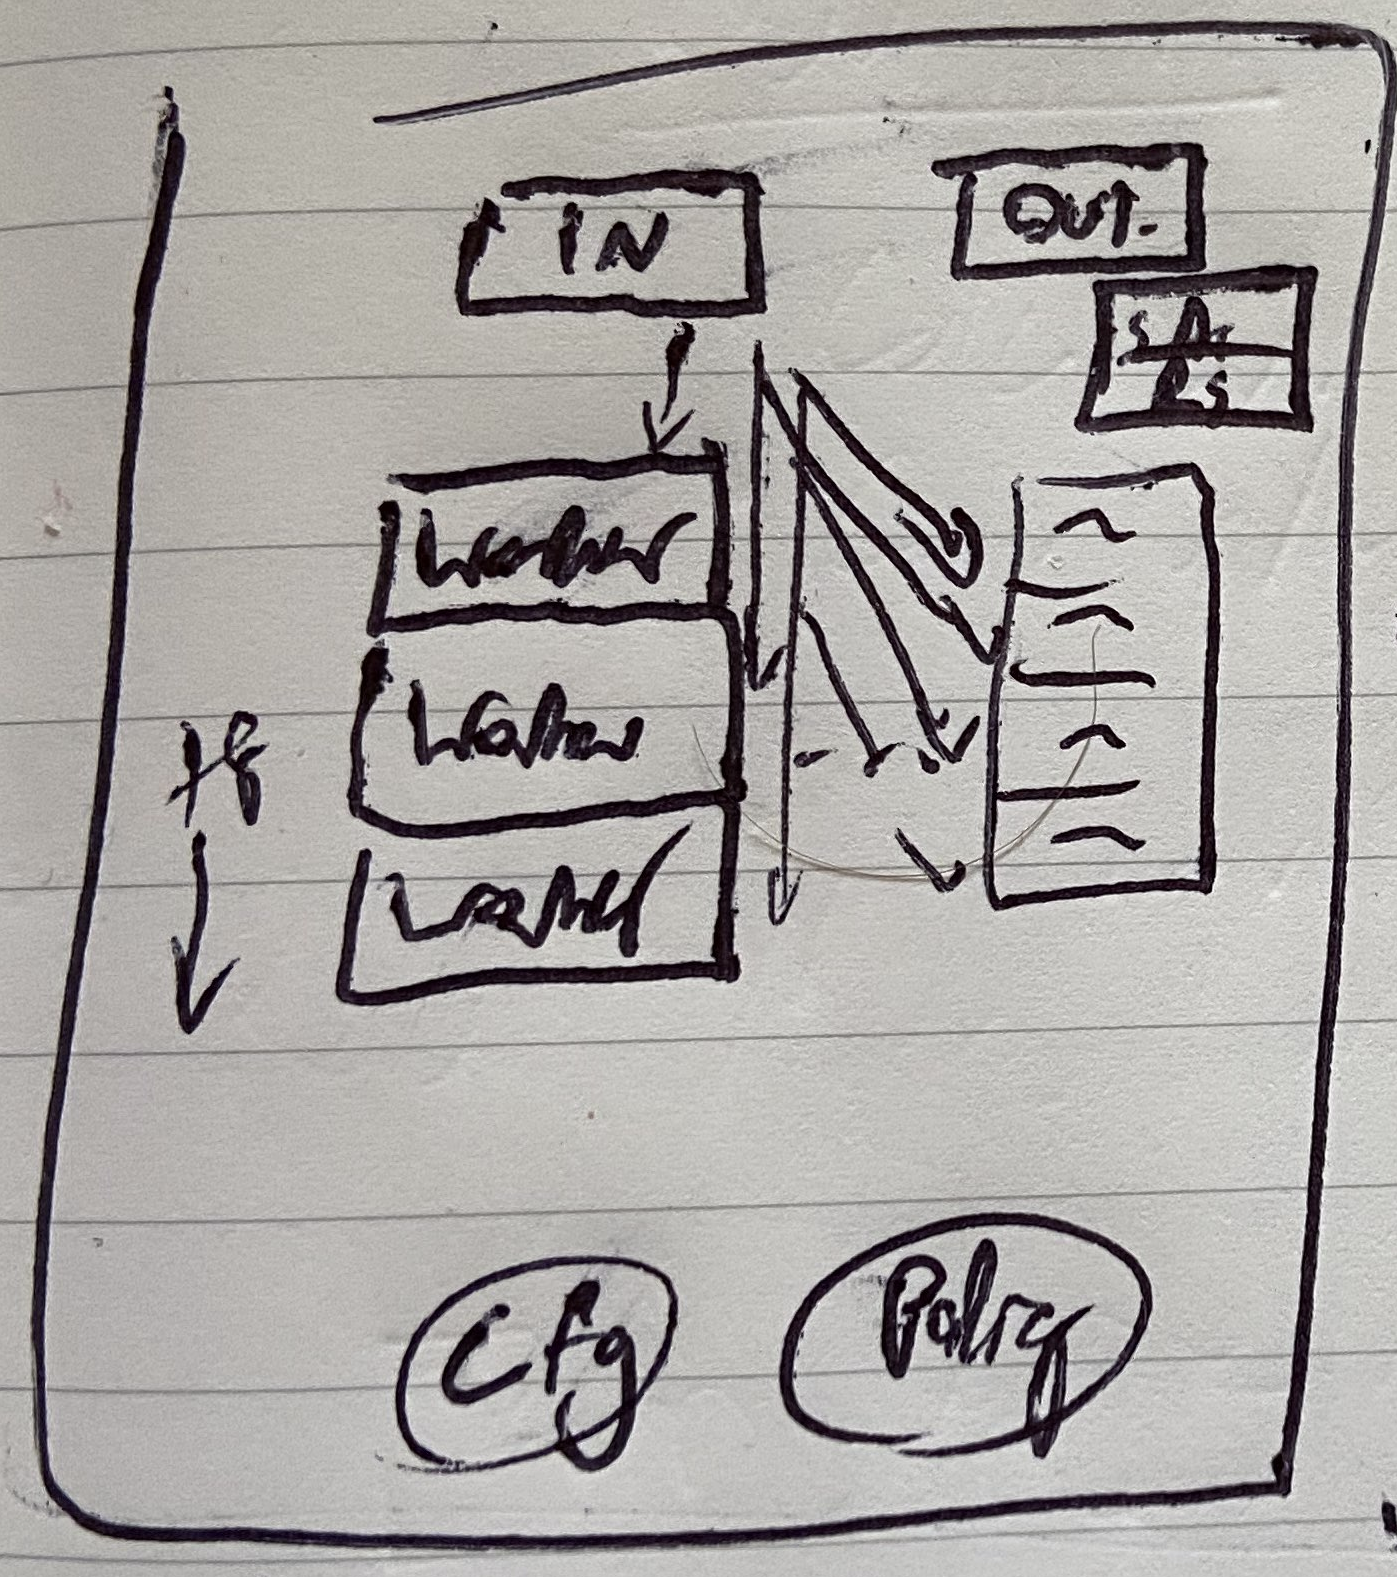
\includegraphics[keepaspectratio, width=\linewidth]{figures/single-core-arch-sketch}
		\caption{Single (offline throughput-optimal).\label{fig:single-and-parallel:single}}
	\end{subfigure}
	\begin{subfigure}{0.45\linewidth}
		\centering
		\includegraphics[keepaspectratio, width=\linewidth]{figures/parallel-arch-sketch}
		\caption{Parallel (online-optimal).\label{fig:single-and-parallel:parallel}}
	\end{subfigure}
	\caption{\approachshort{}'s compute strategies scale to fit device capacity according to latency/throughput needs. ?? MAKE ME FOR REAL \label{fig:single-and-parallel}}
\end{figure}

?? Do we need better/snappier names than just Single/Parallel? It's awfully dry.

In the NFP architecture we use, physical cores (MEs) each have 8 hardware threads (contexts): all contexts on an ME share the same program and employ zero-cost context switches on I/O.
Each core then provides 8 worker threads, though in the parallel case one must be dedicated to monitoring work acknowledgements.
Two main firmware models govern how the computation-intensive parts of these tasks (tile-coding, action preference list construction, policy updates) are carried out:
\begin{description}
	\item[Single (\cref{fig:single-and-parallel:single})] Separate threads listen for new states, and each performs its work sequentially. Computing an action list requires a \emph{read lock} on the policy. If an update occurs, the core requests a \emph{write lock} before updating, greatly limiting online throughput. Tile lists are stored for update computation.
	\item[Parallel (\cref{fig:single-and-parallel:parallel})] Threads cooperate on processing state vectors, minimising latency. Workers have a fixed list of work items, while a master thread sends compute/update commands before awaiting worker completion. Work items are disjoint, requiring no policy locks. State vectors are stored for update computation.
\end{description}
Each offers a different point of optimisation; if updates are disabled, then the \emph{single} model can maximise throughput, while the \emph{parallel} model is designed to minimise decision latency and needs no locks for updating the policy (increasing \emph{online learning} throughput).

We found that, paradoxically, it was more efficient in the parallel case \emph{to do more work} by having each worker recompute its tile subset from a stored state.
It transpired that cacheing this data placed a larger \texttt{memcpy} in the serial section, whose size did not scale at all with bit depth.

\subsection{Agent-Environment Communication}\label{sec:agent-environment-communication}
\approachshort{} uses \emph{multiple-producer/multiple-consumer} (MPMC) messaging channels to communicate with other computational elements; be they P4 programs on the packet path, or additional on-chip analysis and control modules.
Through these channels the system \emph{pushes} state vectors, reward measures, and control/setup packets as its inputs, and \emph{pulls} a stream of state-action pairs as its outputs.
This allows agent decisions to be made asynchronously---preventing packet stalling---and allowing for many parallel decision-making agents to be used if desired.
The key insight of this mechanism is that on-chip reward/state signals enjoy first-class support in much the same manner as packets from the P4 dataplane, allowing agents to act on environmental signals from other on-NIC/chip asynchronous processes or the controller.

Our implementation uses platform-specific IPC mechanisms (\emph{EMEM ring buffers}) with hardware signalling mechanisms on work arrival to achieve this.
Due to the lack of memory allocation in these environments, P4 pipeline threads request buffers for packet payloads using a shared freelist to enable state/configuration/policy data handover.
Packet headers are extracted and parsed using the tooling and data types autogenerated by the P4 pipeline.
We found that this costs a median \SIrange{126}{140}{\nano\second} communication time, comparable to message channels in the Rust and Go languages on commodity hardware.

\subsection{Intra-Agent Communication}
Even with embarrassingly parallel problems, optimising for latency requires meticulous care in how work is passed out and aggregated.
This is truer still when moving from the moderately fine-grained, efficient control of classical RL methods ($\sim$\SI{2}{\milli\second}) to its logical limit (tens of \si{\micro\second}).
Ordinarily, the serialisation/marshalling of requests, responses, and safe shared data access can incur significant extra overheads.
On-chip execution and the nature of action preference computation allow us to use lockless atomic aggregation, removing the overheads of explicit messaging/packetisation.
Moreover, physically adjacent functional units may have special-purpose shared registers or share a small fast cache to accelerate communication further.

Our implementation exploits the locality of threads, cores, and their parent islands in the NFP architecture.
Groups of \numrange{4}{12} cores (MEs) in this platform are termed \emph{islands}, with shared access to low-latency scratch memory and the adjacent registers of neighbouring MEs.
Each ME then has a number of threads fixed at compile time (\numrange{4}{8}), sharing one large register file to enable zero-cost context switches.
Policy compute/update tasks and configuration updates are passed between cores using these direct \emph{next neighbour} registers, signalling all child threads in response.
Each task performs atomic adds to a shared preference list, and atomically increments an acknowledgement counter to be periodically checked by the master thread.

In earlier designs we had experimented with bounded buffers as in \cref{sec:agent-environment-communication} for this, modified to be located solely in local scratch memory, dedicating the master thread to result aggregation.
We found that this created a performance bottleneck at this final stage, causing significant head-of-line blocking for each of the workers.
Similarly, our next neighbour work notification scheme ($\sim$\SI{20}{\nano\second} latency per relayed message) was examined against \emph{reflector} and \emph{work queue} IPC mechanisms (\SIlist{58;126}{\nano\second} per messaged core).
These slower messages can be used in theory to skip ahead into longer ME chains.

\subsection{Reconfigurability}
\approachshort{} allows for policy dimensions, size, action count, tiling strategies, and algorithmic learning parameters ($\alpha, \gamma, \epsilon$, related falloffs) to be chosen and changed at runtime.
This extends to policy data, which may be imported from an offline pre-trained model via such packets, and exported via the NFP binary support package on the host machine.
Some aspects must be chosen at compile time; bit-depth, work allocation strategy, and maximum policy/tiling/state sizes---these govern core operation or allocated memory regions.

In our implementation, configuration packets are carried over UDP and signalled to the P4 parser using a reserved DSCP value as used by \textcite{DBLP:conf/isca/LiLYCSH19}.
While we primarily use this to automate parser generation, this also allows for configuration packets to be received from only trusted hosts over the dataplane if needed via P4 rules.
Our control packet generation library (and evaluation frameworks which build upon it) are written in Rust.

\subsection{Work Allocation}
Due to the lack of dynamic memory allocation and to simplify action-value lookups, policies cannot be effectively stored sparsely.
As a consequence, tiling space requirements scale exponentially with dimension count, and so higher-dimension tilings must be placed in memory regions large enough to allocate space for them.
As a result, tilings are split across memory regions, giving different access and compute costs to different tasks---ranging over CLS, CTM and EMEM in increasing latency.

We use a simple first-fit work placement algorithm run on the NFP, placing the largest work item into the least loaded thread of the least loaded core.
The cost of any individual work item (according to its dimension count and memory location) was estimated offlin.
This work allocation and any cached per-work-item values are recomputed when any configuration is installed or changed.

\subsection{Variable Quantisation Bit Depth}
At compile-time, \approachshort{} can be configured to use \SIlist[list-final-separator = { \translate{or} }]{32;16;8}{\bit} values in input states and its internal policies.
Naturally, smaller bit depths reduce the storage required for policies, tiling data, and stored state-action pairs---allowing more complex problems to be modelled using more dimensions or fine-grained policies.
Through the lens of computational efficiency, reduced bit depth allows action preference lists to be read using fewer I/O operations (as more values may fit into a single machine word).
We had investigated bit-stuffing several such values into a single word for our atomic writeback mechanism (as the platform offers both \SIlist{32;64
}{\bit} atomic addition).
This is analogous to SIMD---through clever use of padding bits---but we found that manipulating tiles into the correct format added \SI{10}{\percent} extra overhead.

\subsection{Notes from chat with Rhys}
?? Where/how to fit this in? I think it's a useful point.

The two compute models discussed here need not be homogeneously deployed.
For instance, in a networked deployment a subset of \approachshort{} nodes could be \SI{32}{\bit} \emph{parallel} agents, training online, while most other nodes ran \SI{8}{\bit} \emph{single} designs to meet throughput guarantees.
The control plane would then be responsible for combining, downsampling, and distributing these improved policies between remaining agents.
This can be taken further still, using policy deltas or execution traces to enable out-of-path transfer learning for more complex function approximators such as neural networks.

%Potential: low-latency train for some specific points, and high throughput for others? Think on the exact note I took...
%
%``can have accel'd offline, train online subset w/ my approach''
%
%THis might mean "do 32-bit online", then downsample to 8-bit policy for high-throughput mode.
%
%Can changes in trained policy be used to transfer to a more complex function approximator elsewhere?

\subsection{Limitations}
Unfortunately, direct rule installation into P4 tables from the SmartNIC itself is not, in general, possible.
To achieve line-rate match-action table lookup, platforms like NFP use accelerated datastructures (e.g., DCFL~\parencite{DBLP:conf/infocom/TaylorT05}) which must be computed by the controller over the \emph{entire rule set}.
Even through externs, 

We instead suggest on NFP chips that externs or datapath stages which apply actions to packet processing should maintain a small local store of state-action pairs, and periodically send these back to the controller for batch rule installation.
This ensures that the vast majority of installed rules enjoy accelerated performance, while preventing rule installation delay on the newest decisions.
Platforms such as Intel Tofino greatly simplify this, with Tofino Native Architecture intrinsics such as \emph{Action Profiles/Selects} allowing a P4 action to be chosen based on a register value (i.e., an RL action).

\subsection{Targeting other device classes}
While this design caters primarily to Netronome's SmartNIC devices, many aspects of this design have clear analogues in NICs of similar form-factor, such as their close NetFPGA SUME cousins.
For instance, the availability of other cores can be handled by designing additional off-path functional units, much like the floating-point adders used by \textcite{DBLP:conf/isca/LiLYCSH19}.
Rather than general-purpose cross-core communication, an RL functional unit would be hard-wired to and from the custom actions that interface with it, using the P4$\rightarrow$NetFPGA toolchain to offer the base framework and granular control over packet and flow selection.
Further optimisations arise from this model: a NetFPGA design would be able to replicate and optimise further on this concept of dedicated, low-latency communication between functional units.
Consider a single, shared, read-only register between RL functional ...
?? think about really really carefully lest Reviewer 2 murder you
?? Parallel, atomic writes at the required resolution.
?? No bit stuffing required for SIMD-alike?.
?? More chances for vectorisation? Is that where we're falling down atm with 32-bit being weirdly optimal?

Bringing this to high-port density devices such as Intel Tofino-powered switches is more difficult.
As discussed in \cref{sec:motivation}, Tofino ASICs map closely to the P4 PSA, meaning that there are no spare asynchronous general-purpose compute units to place this work on.
A potential solution is to divide RL actions across several received packets (i.e., iteratively computing a portion of the action preference list each time) until any further work would delay outbound transmission.
This, however, would introduce new issues surrounding concurrent accesses, work splitting, and altered timescales for learning: we leave their treatment and examination to future work.

%\begin{figure}
%	\centering
%	\resizebox{\linewidth}{!}{\begin{tikzpicture}
%		\node(remote){Remote};
%		
%		%%%
%		
%		\node[below=0.05 of remote](swpos){};
%		\node[fill=white!80!uofgcobalt, draw=black, minimum height=1.5cm, minimum width=2cm, below right= 0.1 of swpos.north west](sw1){};
%		\node[fill=white!80!uofgcobalt, draw=black, minimum height=1.5cm, minimum width=2cm, below right= 0.1 of sw1.north west](sw2){};
%		\node[fill=white!80!uofgcobalt, draw=black, minimum height=1.5cm, minimum width=2cm, below right= 0.1 of sw2.north west](switch){};
%		\node[below right, inner sep=2pt] at (switch.north west) {\small Switch};
%		\node[fill=white!90!uofgcobalt, draw, rectangle, rounded corners=0.05cm, above=0.1] (oswlc) at (switch.south) {\begin{varwidth}{1.5 cm}\small \centering Load\\Collector\end{varwidth}};
%		
%		%
%		
%		\node[right=2 of swpos](epos){};
%		\node[fill=white!80!uofgthistle, draw=black, minimum height=1.5cm, minimum width=3.5cm, below right= 0.1 of epos.north west](e1){};
%		\node[fill=white!80!uofgthistle, draw=black, minimum height=1.5cm, minimum width=3.5cm, below right= 0.1 of e1.north west](e2){};
%		\node[fill=white!80!uofgthistle, draw=black, minimum height=1.5cm, minimum width=3.5cm, below right= 0.1 of e2.north west](egress){};
%		\node[below right, inner sep=2pt] at (egress.north west) {\small Egress Switch};
%		\node[fill=white!90!uofgthistle, draw, rectangle, rounded corners=0.05cm, above=0.1] (eglc) at ($(egress.south) + (-0.85,0)$) {\begin{varwidth}{1.5 cm}\small \centering Load\\Collector\end{varwidth}};
%		\node[fill=white!90!uofgthistle, draw, rectangle, rounded corners=0.05cm, right=0.1] (egest) at (eglc.east) {\begin{varwidth}{1.5 cm}\small \centering Estimator\\$g(\cdot)$\end{varwidth}};
%		
%		%
%		
%		\node[right=3.5 of epos](apos){};
%		\node[fill=white!60!uofgpumpkin, draw=black, minimum height=1.5cm, minimum width=2cm, below right= 0.1 of apos.north west](a1){};
%		\node[fill=white!60!uofgpumpkin, draw=black, minimum height=1.5cm, minimum width=2cm, below right= 0.1 of a1.north west](a2){};
%		\node[fill=white!60!uofgpumpkin, draw=black, minimum height=1.5cm, minimum width=2cm, below right= 0.1 of a2.north west](otheragent){};
%		\node[below right, inner sep=2pt] at (otheragent.north west) {\small Agent vNF};
%		\node[fill=white!90!uofgpumpkin, draw, rectangle, rounded corners=0.05cm, above=0.3] (oasa) at (otheragent.south) {\begin{varwidth}{1.5 cm}\small \centering Stats API\end{varwidth}};
%		
%		%
%		
%		\node[below=2.3 of remote.west](linestart){};
%		\path let \p1 = (linestart) in node (lineend) at (9,\y1){};
%		\draw [dashed] (linestart) -- (lineend);
%		
%		%%%
%		
%		\node[below=2.4 of remote](local){Local};
%		
%		%%%
%		
%		\node[below=0.25 of local](aswpos){};
%		\node[fill=white!80!uofgthistle, draw=black, minimum height=3cm, minimum width=2.2cm, below right= 0.1 of aswpos.north west](aswitch){};
%		\node[below right, inner sep=2pt] at (aswitch.north west) {\small Agent Switch};
%		\node[fill=white!90!uofgthistle, draw, rectangle, rounded corners=0.05cm, above=0.1] (aswoft) at (aswitch.south) {\begin{varwidth}{1.5 cm}\small \centering OpenFlow\\Tables\end{varwidth}};
%		\node[fill=white!90!uofgthistle, draw, rectangle, rounded corners=0.05cm, above=0.1] (aswsc) at (aswoft.north) {\begin{varwidth}{1.5 cm}\small \centering Stats\\Collector\end{varwidth}};
%		\node[fill=white!90!uofgthistle, draw, rectangle, rounded corners=0.05cm, above=0.1] (aswlc) at (aswsc.north) {\begin{varwidth}{1.5 cm}\small \centering Load\\Collector\end{varwidth}};
%		
%		%
%		
%		\node (avfpos) at ($(aswpos) + (3,0.2)$){};
%		\node[fill=white!60!uofgpumpkin, draw=black, minimum height=3.5cm, minimum width=4.5cm, below right= 0.1 of avfpos.north west](avf){};
%		\node[below right, inner sep=2pt] at (avf.north west) {\small Agent vNF};
%		\node[fill=white!90!uofgpumpkin, draw, rectangle, rounded corners=0.05cm, below=0.15] (avfsa) at ($(avf.north) + (0.2,0)$) {\begin{varwidth}{1.5 cm}\small \centering Stats API\end{varwidth}};
%		\node[fill=white!90!uofgpumpkin, draw, rectangle, rounded corners=0.05cm, below=0.9] (avfdb) at (avfsa.south west) {\begin{varwidth}{1.5 cm}\small \centering Flowstate\\Database\end{varwidth}};
%		\node[fill=white!90!uofgpumpkin, draw, rectangle, rounded corners=0.05cm, right=0.1] (avfsched) at (avfdb.east) {\begin{varwidth}{1.5 cm}\small \centering TRS\\Scheduler\end{varwidth}};
%		\node[fill=white!90!uofgpumpkin, draw, rectangle, rounded corners=0.05cm, below=2.3] (avfcore) at (avfsa.south) {\begin{varwidth}{1.5 cm}\small \centering Core\end{varwidth}};
%		\node[fill=white!90!uofgpumpkin, draw, rectangle, rounded corners=0.05cm, right=0.8] (avfrl) at (avfcore.east) {\begin{varwidth}{1.5 cm}\small \centering RL\end{varwidth}};
%		
%		%%%
%		
%		\tikzset{>=stealth}
%		
%		\draw[thick, ->] (aswlc) -- (avfsa.west) node[midway,above] {\tiny Current load};
%		\draw[thick, ->] (aswsc) -- (avfsa.west) node[midway,sloped, above] {\tiny Flow stats};
%		
%		\draw[thick, ->] (oswlc) -- (avfsa) node[midway,above, sloped] {\tiny Current load};
%		
%		\draw[thick, ->] (eglc) -- (avfsa) node[midway,above, sloped] {\tiny Current load};
%		\draw[thick, ->] (egest) -- (avfsa) node[midway,above, sloped] {\tiny Estimation data};
%		
%		\draw[thick, <->] (oasa) -- (avfsa) node[midway,above, sloped] {\tiny Experience};
%		
%		\draw[thick, ->] (avfsa) -- (avfdb) node[midway,above, sloped] {\tiny State};
%		\draw[thick, ->] (avfsa) -- (avfsched) node[midway,above, sloped] {\tiny Live flows};
%		
%		\draw[thick, ->] (avfcore) -- (aswoft) node[midway,above, sloped] {\tiny Packet drop rules};
%		\draw[thick, <->] (avfcore) -- (avfdb) node[midway,below, sloped] {\tiny State};
%		\draw[thick, <->] (avfcore) -- (avfsched) node[midway,below, sloped] {\tiny Work};
%		\draw[thick, <-] ($(avfcore.east) + (0,0.1)$) -- ($(avfrl.west) + (0,0.1)$) node[midway,above, sloped] {\tiny Actions};
%		\draw[thick, ->] (avfcore) -- (avfrl) node[midway,below, sloped] {\tiny State};
%		
%		\draw[thick, ->] (avfsa.east) to [out=0, in=45] (avfrl.north);
%		\node[right=0.3] at (avfsa.east) {\tiny Experience};
%		\end{tikzpicture}}
%	\caption{
%		System architecture  for our RL-driven DDoS defence system.
%		\label{fig:sys-arch}
%	}
%\end{figure}

\section{Potential Integrations}\label{sec:potential-integrations}
To show the general applicability and use of \approachshort{}, we propose two ideal integrations which would benefit most from in-NIC reinforcement learning; online DDoS attack mitigation (\cref{sec:integ-1}), and ?? OTHER THING (\cref{sec:integ-2}).
We support these using other state-of-the-art P4/PDP developments.

\subsection{DDoS Defence}\label{sec:integ-1}
?? Link to my own work
?? Explain how every part may be substituted

?? Bump-in-the-wire at edge nodes.

?? How does increased attack flow ratio affect the RL core? How does changing its params to increase its own throughput?
?? Remember the timed-random-selection; use the state coalescing trick indep discovered by you and those other guys.

?? Can the P4 dataplane be used to reduce/increase the number of flows used as inputs? (YES)

?? Place Dapper~\parencite{DBLP:conf/sosr/GhasemiBR17} on the datapath as the main source of state vectors.

?? Use the TNSM work you reviewed~\parencite{tnms-ddos-victim-ident} as a reward function source.

\subsection{Something host-specific?}\label{sec:integ-2}
Accelerate something at an end-host... Flow control? Something datacentre-y? A novel CCA? What?

\section{Evaluation}\label{sec:evaluation}
We outline our performance evaluation of...

?? find something meaningful to put here.

\subsection{Experimental Setup}
Evaluation of \approachshort{} was performed on server blades hosting a single Netronome Agilio LX 1x100GbE SmartNIC (NFP-6480, \SI{1.2}{\giga\hertz}).
These ran Ubuntu 18.04.5 LTS (4.15.0-140-generic x86\_64) on Intel Xeon Bronze 3204 CPUs (\SI{1.9}{\giga\hertz}) and \SI{32}{\gibi\byte} RAM.
Control programs were built using rustc 1.51.0.
We run \approachshort{} on an island with \num{4} MEs of the NFP-6480 for a total of \num{32} hardware threads.
This is the maximum number of MEs on a single island which is not in use by an existing P4 pipeline.
Where feasible, we test \SIlist{32;16;8}{\bit} quantised arithmetic firmware versions.
All timing and throughput measurements were repeated over \num{5000} trials.

Policy sizes are set to those matching a real-world DDoS control application~\parencite{DBLP:journals/tnsm/SimpsonRP20}: 20-dimension state vectors, a bias tile and 16 full tiling sets (7$\times$1-dim, 8$\times$2-dim, 1$\times$4-dim), 8 tilings per dimension set, 6 tiles per dimension, choosing between 10 actions.

Studies based on \textcite{DBLP:journals/tnsm/SimpsonRP20} mirror their experimental setup (Ubuntu 18.04.2 LTS (4.4.3-040403-generic x86\_64), Intel Core i7-6700K (\SI{4.2}{\giga\hertz}), \SI{32}{\gibi\byte} RAM).

\subsection{Experiments}

\fakepara{Raw inference and learning performance}
We compare how long it takes for \approachshort{} to compute actions and update its policy per state vector received, and report on the observed throughput of our designs.
We compare these against floating point and quantised implementations running on a commodity host machine.
This allows us to demonstrate the performance differences between the \emph{Single} and \emph{Parallel} configurations, particularly in how \emph{Single's} required policy locks impact throughput.
We also report on the derived throughput measures accounting for the locking behaviour of each.

Building on this, we vary the amount of allocated worker threads to show how \approachshort{} can scale to fit available compute resources on a device.
This also demonstrates the number of cores needed to achieve a given latency bound on a policy of representative complexity.
Moreover, to demonstrate how these costs vary as policy complexity increases, we vary the number of total dimensions included in the tiling.

?? NOT GOT OTHERS TO COMPARE AGAINST YET, JUST SELF.
?? Mention versus DNN latency in passing here?

\fakepara{Work allocation}
%?? Also our simple, ahead-of-time, work scheduler.
We verify that our heuristic, runtime work scheduler (\emph{Balanced}) makes meaningful use of the explicit memory hierarchy and cost of each work item.
We compare it versus several baselines: a \emph{Na\"{i}ve} chunked scheduler, a \emph{Random} baseline allocation, and a simple \emph{Modular} allocator (where a worker $j$ out of $w$ takes $k$ items given by $\mathit{work}_j=\left\{\left(j + i \times w\right) \bmod n_{\mathit{items}} \mid i \in [0,k) \right\}$).

\fakepara{End-to-end RL latency}
We compare the key RL decision-making latencies we discuss in \cref{fig:state-slip} ($t_1,t_2,t_3$) across 3 scenarios: completely in-NIC (\approachshort{}), offloading RL decisions to a SmartNIC's controller machine, and offloading to the controller of an OpenFlow-compatible switch (OvS).

?? NOT DONE YET
?? MOSTLY A PAPER EXERCISE FROM SOME OTHER MEASURES

\fakepara{Co-existence with the dataplane}
We measure maximum packet rate and bandwidth throughput of a P4 pipeline on our SmartNICs, both with and without \approachshort{}.
This allows us to quantify whether on-chip (out-of-path) execution impacts ordinary dataplane behaviour through indirect means: e.g., EMEM cache evictions or hidden resource contention.
In particular, we stress test both decisions and policy updates of our \emph{Parallel} design at full throughput.

?? NOT DONE YET.

\fakepara{Resource requirements}
Using the maximum policy size defined above, we investigate how the memory requirements imposed by \approachshort{} vary with the number of dedicated MEs, over and above a base P4 forwarding plane.

?? Not done yet: read these out from the IDE.

\fakepara{The impact of bit depth}
We further investigate how bit depth affects the accuracy of policy by varying the number of bits used to represent the mantissa of action values and input state.

\subsection{Results and Discussion}\label{sec:results}

\begin{table}
	\caption{Throughput and per-item compute time for an RL agent with/without policy learning. State$\rightarrow$action latency equals the offline completion cost. TODO: compare to host machine? Put completion times first? Put multi first?}
	\resizebox{\linewidth}{!}{
		\expandableinput ../tables/build/latency-tput
	}
\end{table}

\begin{figure}
	\resizebox{1.0\linewidth}{!}{
		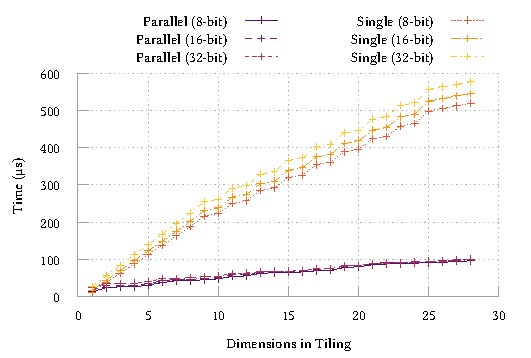
\includegraphics{../plots/build/rl-perf-tester/vary-work}
	}
	\caption{?? More work means More time. ?? Max Parallelisation. ?? Bitdepth affects independent cores more. ?? latency version in appendix: \Cref{fig:vary-work-latency}}
\end{figure}

\begin{figure}
	\resizebox{1.0\linewidth}{!}{
		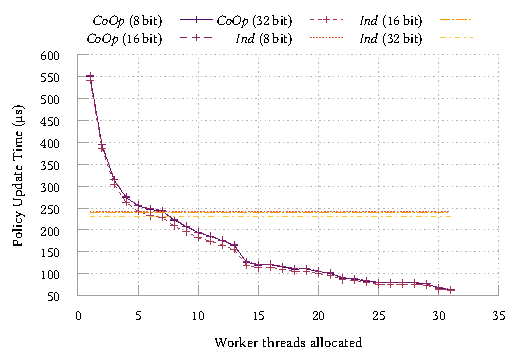
\includegraphics{../plots/build/rl-perf-tester/vary-core}
	}
	\caption{?? More cores means less time ?? Max-size work (129 work-items). ?? Need to dedicate 3 worker to beat independent cores. ?? Sharper perf increase when new physical core added. ?? up to 31 due to master thread. ?? latency version in appendix: \Cref{fig:vary-core-latency}}
\end{figure}

\fakepara{Raw inference and learning performance}
TEST

\fakepara{Work allocation}
?? \Cref{fig:work-alloc-32}

\begin{figure}
	\resizebox{1.0\linewidth}{!}{
		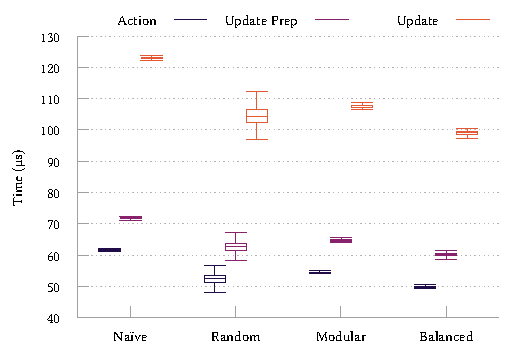
\includegraphics{../plots/build/rl-perf-tester/work-strat-32bit}
	}
	\caption{?? Choice of work strategy is pretty important I guess\label{fig:work-alloc-32}}
\end{figure}

\fakepara{End-to-end RL latency}
TEST

\fakepara{Co-existence with the dataplane}
TEST

\fakepara{Resource requirements}
?? \Cref{tab:resources}

\begin{table}
\caption{NFP memory use due to \approachshort{}. CLS and CTM are shared between all programs on the same island (placing our RL agent on i5), while EMEM and IMEM are shared between all NFP programs on a NIC.\label{tab:resources}}
\resizebox{\linewidth}{!}{
\begin{tabular}{@{}cSSSSSSSSSS@{}}
	\toprule Firmware & \multicolumn{2}{c}{EMEM} & \multicolumn{2}{c}{EMEM Cache} & \multicolumn{2}{c}{IMEM} & \multicolumn{2}{c}{i5.CLS} & \multicolumn{2}{c}{i5.CTM}\\
	& \multicolumn{1}{c}{\si{\mebi\byte}} & \multicolumn{1}{c}{\si{\percent}} & \multicolumn{1}{c}{\si{\kibi\byte}} & \multicolumn{1}{c}{\si{\percent}} & \multicolumn{1}{c}{\si{\kibi\byte}} & \multicolumn{1}{c}{\si{\percent}} & \multicolumn{1}{c}{\si{\kibi\byte}} & \multicolumn{1}{c}{\si{\percent}} & \multicolumn{1}{c}{\si{\kibi\byte}} & \multicolumn{1}{c}{\si{\percent}} \\
	\midrule Base P4 & 6794.73 & 88.47 & 0 & 0 & 858.28 & 10.48 & 0 & 0 & 0 & 0 \\
	Single (1-core) & 6778.83 & 88.27 & 1737.91 & 18.86 & 1263.28 & 15.42 & 28.69 & 44.82 & 90 & 35.16 \\
	Single (4-core) & 0 & 0 & 0 & 0 & 0 & 0 & 0 & 0 & 0 & 0 \\
	Parallel (1-core) & 0 & 0 & 0 & 0 & 0 & 0 & 0 & 0 & 0 & 0 \\
	Parallel (4-core) & 0 & 0 & 0 & 0 & 0 & 0 & 0 & 0 & 0 & 0 \\
	\bottomrule
\end{tabular}
}
\end{table}

\fakepara{The impact of bit depth}
?? \Cref{fig:quant-acc}

\begin{figure}
	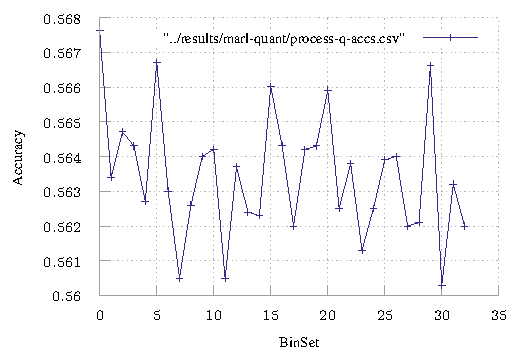
\includegraphics{../plots/build/marl-quant/accuracy-binary}
	\caption{Normalised accuracy of a converted, pre-trained floating-point tile-coded policy after conversion to $32Qn$ fixed-point.}\label{fig:quant-acc}
\end{figure}

\section{Related Work}

?? A switch/NIC architecture like \textcite{DBLP:conf/hotnets/StephensAS18} would remove the need for hard-coded island-island relationships.

?? Event-driven model could better support many timer-driven RL use-cases \textcite{DBLP:conf/hotnets/IbanezABM19}.

?? Taurus. They can't train online though!~\parencite{DBLP:journals/corr/abs-2002-08987}

?? Do switches~\parencite{DBLP:conf/hotnets/XiongZ19}.
?? Train offline, classical methods targetting all match-action P4 systems (no externs etc).

?? N3IC run NNs on NIC~\parencite{DBLP:journals/corr/abs-2009-02353}, allow packet tagging to occur based on pre-trained BNN~\parencite{DBLP:conf/nips/HubaraCSEB16}.
?? both NFP and NetFPGA.
?? Or as an offload mechanism~\parencite{DBLP:conf/sigcomm/SanvitoSB18,DBLP:journals/corr/abs-1801-05731}.
?? Binary NNs ``more suitable for network hardware''~\parencite{DBLP:journals/corr/MiyashitaLM16}?

?? Can we collect some papers on per-packet ML/RL? Per-packet classification using NNs to build decision trees~\parencite{DBLP:conf/sigcomm/LiangZJS19}

?? RL for congestion control. ~\parencite{DBLP:journals/corr/abs-1910-04054}

?? Arbitrary training enhanced by in-network? General NNs~\parencite{DBLP:conf/micro/LiPAYQPWSEK18}, RL-specfic~\parencite{DBLP:conf/isca/LiLYCSH19}.

?? Mechanisms to support full in-switch DDoS detection~\cite{tnms-ddos-victim-ident}.

\section{Conclusion}

\begin{acks}
	The authors would like to thank Rhys Simpson for his comments and discussions on SIMD-like optimisations.
	This work was supported in part by the \grantsponsor{gs-epsrc}{Engineering and Physical Sciences Research Council}{https://epsrc.ukri.org/} [grant~\grantnum{gs-epsrc}{EP/N509668/1}].
\end{acks}
	
%\bibliographystyle{ACM-Reference-Format}
%\bibliography{reference}
\printbibliography

\begin{appendices}
	\section{Old ``What could we do``?}
	How do we evaluate this without looking into classification performance?
	\begin{itemize}
		\item Analytically?
		\begin{enumerate}
			\item Prove that tile splitting scheme over memory hierarchy can improve performance.
			\begin{itemize}
				\item Hit rate of different tiles according to tile dimensionality?
				\item Access time for each tier of memory hierarchy.
			\end{itemize}
		\end{enumerate}
		\item Experimentally?
		\begin{enumerate}
			\item Create ``VNF'' testbed: mirror traffic from switch to a host for telemetry processing/flow state. Send flow state over to another node who computes RL actions. RL actions installed on switch.
			\begin{itemize}
				\item Why not co-host RL computation with telemetry? Could be separate functions, could want to ensure that neither impacts the performance of the other.
			\end{itemize}
			\item Create ``PDP'' testbed: Load firmware, pass in traffic. Traffic processing/action compute/table mod occurs in PDP.
			\item What traffic? Healthy mix of attack (UDP), Discord legit Opus VoIP traffic, HTTP bulk-transfer traffic.
			\item Measure $t_{1 \cdots 3}$ according to \cref{fig:state-slip} in both VNF and PDP contexts.
			\begin{description}
				\item[$t_1$]
				\begin{description}
					\item[PDP] Packet ingress $\rightarrow$ INT Island $\rightarrow$ State arrival in Control ME.
					\item[VNF] Packet mirror time $\rightarrow$ telemetry VNF $\rightarrow$ state arrival in agent vnf.
				\end{description}
				
				\item[$t_2$]
				\begin{description}
					\item[PDP] Time to compute action over parallel Policy MEs (RL Island, SmartNIC).
					\item[VNF] Time to compute action in host program (on VNF) from received state.
				\end{description}
				
				\item[$t_3$]
				\begin{description}
					\item[PDP] Modify local tables across ME/Island boundaries (same device), verify rule present (or get ACK).
					\item[VNF] Generate OpenFlow control messages, send OF message to switch, verify rule present (or get ACK).
				\end{description}
			\end{description}
			\item HYPOTHESIS: PDP will present a reduction in these three times for per-flow state.
			\item QUESTION: Does same apply to learning?
			\item NOTE: since we're not actually assessing the \emph{quality} of output decisions, we can cut corners on what data is sent out and where. I.e., in-band network telemetry island can be skipped, if we move over representative volumes of state to/from the RL island with approximately correct delay as recorded by other studies.
		\end{enumerate}
	\end{itemize}
	I can think of one way to evaluate this if we employ classification performance:
	\begin{enumerate}
		\item Run the existing work~\parencite{DBLP:journals/tnsm/SimpsonRP20}, acquire a policy for one node after full info sharing.
		\item Load this policy onto the RL Island (\cref{fig:netro-arch}).
		\item Either feed in raw state packets, or feed in traffic if we can get INT working.
		\item For each level of quantisation needed, examine average performance.
		\item Don't compare against old numbers for final perf: use a ``VNF'' setup similar to above---this will probably suffer a bit compared to old results, where everything was on the same machine. Make it relative/normalised.
	\end{enumerate}

	\section{Intermediate steps?}
	System?
	\begin{itemize}
		\item Setup other core as event source.
		\begin{itemize}
			\item \emph{\num{2} week.}
			\item Idea: proxy for idea of INT core mentioned elsewhere, combined with the main periodic event sending that the last RL work relied upon. So, say "you can put that state management and extraction on another core, here's what the comms cost is" or similar.
		\end{itemize}
		\item Fixes to hash table use, signalling.
		\begin{itemize}
			\item \emph{\num{1} week.}
			\item Blocks progress on optimisation, correct multi-stream RL.
		\end{itemize}
		\item Optimise/parallelise action compute/learning.
		\begin{itemize}
			\item \emph{\num{2} week.}
			\item Value? Proves this approach can scale according to resource availability/demand on the deployment device, at compile-time anyhow.
		\end{itemize}
	\end{itemize}
	
	Experiments?
	\begin{itemize}
		\item Measure sum of times $t_{1...3}$ described elsewhere.
		\begin{itemize}
			\item \emph{\num{1} week.}
			\item Currently have individual, need ``end-to-end''.
		\end{itemize}
		\item Throughput impact testing.
		\begin{itemize}
			\item \emph{\num{1} week.}
			\item Requires current impl, creation of basic testbed and packet forwarding setup.
			\item Use-case independent.
		\end{itemize}
		\item Measure execution, training costs for varying policy sizes.
		\begin{itemize}
			\item \emph{\num{1.5} weeks.}
			\item Policies need not be meaningful, and can be garbage data. Use-case independent.
			\item Partially blocked on multicore accelerated/optimised execution.
		\end{itemize}
		\item Measure rule installation cost on different platforms.
		\begin{itemize}
			\item \emph{\num{1.5} weeks.}
			\item Blocked on creation of basic testbed and packet forwarding setup.
		\end{itemize}
		\item Investigate stationarity.
		\begin{itemize}
			\item \emph{\numrange{2}{3} weeks.}
			\item Requires full use-case implementation.
			\item Requires careful thought about sensible changes to normality.
			\item Might be bolstered by comparison against an offline-trained system?
		\end{itemize}
	\end{itemize}
	
	\section{Everything we could possibly evaluate}
	
	Evaluation will need to be divided into 2 main categories:
	\begin{enumerate}
		\item Simulation/emulation based on mininet.
		\begin{itemize}
			\item These can only assess algorithmic properties, as performance measurements in mininet (i.e., a full mult-agent system) are not representative.
		\end{itemize}
		\item Testbed setup (2/3 configurations):
		\begin{itemize}
			\item These will assess key system performance properties of a \emph{single agent}, in control of a single switch/NIC as a bump in the wire. Bump-in-the-wire device will carry traffic between two hosts.
			\item \emph{Time permitting, may need to send state vectors in packets rather than do feature/state extraction on-chip}.
			\item \emph{Necessary.} RL runs on bump-in-the-wire SmartNIC.
			\item \emph{Either/both.} P4-based off-path RL. Custom packet actions (e.g., random drop) will be implemented in P4 with externs. Packets/digests mirrored to state extraction machine. Agent may be co-hosted with state-extraction. Rules inserted via P4-device specific RTE.
			\item \emph{Either/both.} OvS-based off-path RL. Custom packet actions are already implemented in OvS as OpenFlow extensions. Packets/digests mirrored to state extraction machine. Agent may be co-hosted with state-extraction.
		\end{itemize}
	\end{enumerate}
	
	\subsection{What is this different from, or better than?}
	List below mainly for the benefit of helping enumerate everything I can compare against, and what their drawbacks are.
	
	\begin{itemize}
		\item (Deep) neural network-backed RL.
		\begin{itemize}
			\item NNs infeasible to update online. Ordinarily this requires larger volumes of data than can be gathered in real time, but becomes substantially more difficult after change of representation (quantisation, binarisation). An online system (such as this) should be able to adapt to changes in underlying traffic, optimisation criteria, etc., dynamically.
			\item Complexity of function approximation means that policy updates are more computationally complex to compute. For instance, NNs require use of the backpropagation algorithm, rather than the simpler classical schemes which need only the tile set already identified in action selection.
			\item Only heavily quantised (i.e., binary neural networks) suitable for in-switch execution.
		\end{itemize}
		
		\item MARL and other ``agents as network functions'' designs.
		\begin{itemize}
			\item Action, state collection, updates etc. happen on nodes outside of the main packet path in this paradigm. Thus, state measurements, action computation, and so on, should induce the state drift described above. Also makes these approaches ``slower to react'' in theory.
		\end{itemize}
	\end{itemize}
	
	At present, there are no other RL works in PDPs, let alone with online policy updates.
	Other existing RL use cases suitable for adaptation to the ``bump-in-the-wire'' model are proving tricky to find.
	
	\subsection{Emulation metrics}
	Key (MVP) metrics will be \textbf{bolded}, and expanded with a subsubsection.
	
	\textbf{Quantisation accuracy}, quantised training accuracy, \textbf{stationarity}.
	
	\subsubsection{Quantisation accuracy}
	Examination of whether lower resolution quantisation impacts RL agent decision accuracy substantially.
	
	This has been done using MARL in mininet, see \cref{fig:quant-acc}.
	
	\subsubsection{Interaction with stationarity}
	Learning time of the system as compared to known changes in normality.
	
	I.e., in the DDoS case: how long does an agent take to respond to the onset of an attack?
	A change in attack strategy?
	The conclusion of an attack?
	There are no citations on \emph{how} DDoS attacks evolve, just that they do, and that this can occur on various timescales.
	
	\subsection{Testbed metrics}
	Key (MVP) metrics will be \textbf{bolded}, and expanded with a subsubsection.
	
	\textbf{Traffic throughput (bytes, packets)}, \textbf{packet processing delay}, \textbf{action execution time}, \textbf{learning time}, from-scratch learning accuracy, \textbf{rule installation delay/cost}, host and NIC memory costs, policy installation time, ``accuracy'' in the DDoS case.
	
	\subsubsection{Traffic throughput}
	Main research question: does moving RL logic onto the NIC reduce maximum throughput of the NIC, even if calculation is on a different functional unit?
	This is relevant in both \si{\byte\per\second} and packets per second.
	
	This is application independent, and would assess whether the RL units (acting independently on the netronome) affect throughput compared with a basic P4 program at different work intensities.
	Ideally, this would show no effect on forwarding performance.
	
	\subsubsection{Packet processing delay}
	Main research question: does the presence of off-path (but on-chip) RL execution meaningfully increase packet processing delay? How does this compare to a P4 program with an equivalent number of tables? What about to OvS?
	
	\subsubsection{Action execution \& learning time}
	Main research question: does moving RL logic from the host to the NIC substantially reduce delays from state measurement, to state receipt, to action computation and installation?
	These constitute $t_{1...3}$ discussed above.
	Primarily, these need to be looked at using varying policy sizes and distribution across memory regions.
	
	We ideally want these both with and without any acceleration from extra cores on the netronome: the point of this being that we can demonstrate that the system (or a similar NetFPGA system) can scale upwards according to available system resources or demands.
	
	\subsubsection{Rule installation delay/cost.}
	Main research question: how long does it take to install rules in the above testbed setups? What is the downtime of so doing?
	
	This is application-dependent: see earlier discussions on rule batching and local extern/hash-table use.
	
	\begin{figure}
		\resizebox{1.0\linewidth}{!}{
			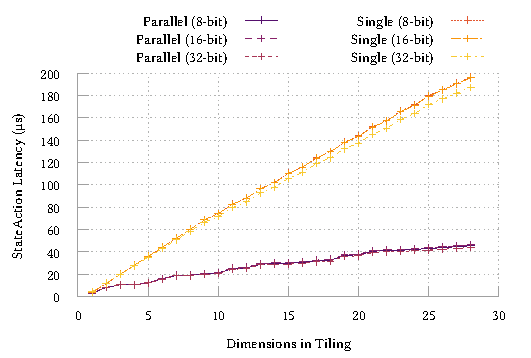
\includegraphics{../plots/build/rl-perf-tester/vary-work-latency}
		}
		\caption{Latency! varying work.\label{fig:vary-work-latency}}
	\end{figure}
	
	\begin{figure}
		\resizebox{1.0\linewidth}{!}{
			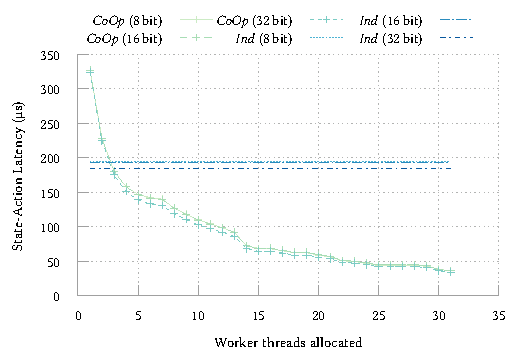
\includegraphics{../plots/build/rl-perf-tester/vary-core-latency}
		}
		\caption{Latency! varying core count\label{fig:vary-core-latency}}
	\end{figure}
\end{appendices}

	
\end{document}